\documentclass[twoside,twocolumn,10pt]{extarticle}

\usepackage{multirow}
\usepackage{textcase}
\usepackage{amsthm}
\usepackage{amssymb}
%\newtheorem{thm}{Theorem}
\theoremstyle{definition}
%\newtheorem{defn}[thm]{Definition} % definition numbers are dependent on theorem numbers
%\newtheorem{exmp}[thm]{Example}

\usepackage{blindtext} % Package to generate dummy text throughout this template 

\usepackage[sc]{mathpazo} % Use the Palatino font
\usepackage[T1]{fontenc} % Use 8-bit encoding that has 256 glyphs
\linespread{1.05} % Line spacing - Palatino needs more space between lines
\usepackage{microtype} % Slightly tweak font spacing for aesthetics

\usepackage[italian]{babel} % Language hyphenation and typographical rules
\usepackage[utf8]{inputenc}

\usepackage[hmarginratio=1:1,top=32mm,columnsep=20pt]{geometry} % Document margins
\usepackage[hang,small,labelfont=bf,up,textfont=it,up]{caption} % Custom captions under/above floats in tables or figures
\usepackage{booktabs} % Horizontal rules in tables
\usepackage{subcaption}

\usepackage{graphicx}
\usepackage{float}
\usepackage{listings}
\usepackage{color}
\usepackage{textcomp}

\definecolor{codegreen}{rgb}{0,0.6,0}
\definecolor{codegray}{rgb}{0.5,0.5,0.5}
\definecolor{codepurple}{rgb}{0.58,0,0.82}
\definecolor{backcolour}{rgb}{0.95,0.95,0.92}

\lstdefinestyle{mystyle}{
	backgroundcolor=\color{backcolour},   
	commentstyle=\color{codegreen},
	keywordstyle=\color{magenta},
	numberstyle=\tiny\color{codegray},
	stringstyle=\color{codepurple},
	basicstyle=\footnotesize,
	breakatwhitespace=false,         
	breaklines=true,                 
	captionpos=b,                    
	keepspaces=true,                 
	numbers=left,                    
	numbersep=5pt,                  
	showspaces=false,                
	showstringspaces=false,
	showtabs=false,                  
	tabsize=2
}
\lstset{style=mystyle}

\usepackage{lettrine} % The lettrine is the first enlarged letter at the beginning of the text

\usepackage{enumitem} % Customized lists
\setlist[itemize]{noitemsep} % Make itemize lists more compact

\usepackage{abstract} % Allows abstract customization
\renewcommand{\abstractnamefont}{\normalfont\bfseries} % Set the "Abstract" text to bold
\renewcommand{\abstracttextfont}{\normalfont\small\itshape} % Set the abstract itself to small italic text

\usepackage{titlesec} % Allows customization of titles
\renewcommand\thesection{\Roman{section}} % Roman numerals for the sections
\renewcommand\thesubsection{\roman{subsection}} % roman numerals for subsections
\titleformat{\section}[block]{\large\scshape\centering}{\thesection.}{1em}{} % Change the look of the section titles
\titleformat{\subsection}[block]{\large}{\thesubsection.}{1em}{} % Change the look of the section titles

\usepackage{fancyhdr} % Headers and footers
\pagestyle{fancy} % All pages have headers and footers
\fancyhead{} % Blank out the default header
\fancyfoot{} % Blank out the default footer
\fancyhead[C]{Apprendimento per Rinforzo $\bullet$ Maggio 2017 $\bullet$ \textit{Machine Leargning}} % Custom header text
\fancyfoot[RO,LE]{\thepage} % Custom footer text

\usepackage{titling} % Customizing the title section

\usepackage{hyperref} % For hyperlinks in the PDF

% Title Section
\setlength{\droptitle}{-4\baselineskip} % Move the title up

\pretitle{\begin{center}\Huge\bfseries} % Article title formatting
\posttitle{\end{center}} % Article title closing formatting
\title{Reinforcement Learning e\\ Agenti basati su Experience Replay:\\ Caso di Studio di Inefficacia} % Article title
\author{%
\textsc{Maxim Gaina e Bartolomeo Lombardi} \\[1ex] % Your name
\normalsize Università di Bologna\thanks{Progetto per il corso di Complementi di Linguaggi di Programmazione, A.A. 2016/2017, prof. Andrea Asperti.} \\ % Your institution
\normalsize \href{mailto:maxim.gaina@studio.unibo.it}{\{maxim.gaina, bartolomeo.lombardi\}@studio.unibo.it}
%\and % Uncomment if 2 authors are required, duplicate these 4 lines if more
%\textsc{Jane Smith}\thanks{Corresponding author} \\[1ex] % Second author's name
%\normalsize University of Utah \\ % Second author's institution
%\normalsize \href{mailto:jane@smith.com}{jane@smith.com} % Second author's email address
}
\date{\today} % Leave empty to omit a date
\renewcommand{\maketitlehookd}{%
\begin{abstract}
\noindent Data la rete neurale Deep Q\texttwelveudash Network ideata e implementata da DeepMind, l'obiettivo di questo lavoro di progetto consiste nel comprendere per quale motivo tale agente, in breve DQN, ha ottenuto risultati sotto la soglia delle prestazioni umane su un sottoinsieme del parco giochi Atari 2600. Verrà quindi studiato l'Apprendimento per Rinforzo, il modello Experience Replay e l'architettura delle reti neurali sottostanti; pur non disponendo delle stesse risorse di calcolo, verranno fatte delle prove pratiche in grado di mimare i risultati ottenuti precedentemente, analizzandoli. Infine si cercherà di dare uno sguardo a quali sono state le innovazioni in questo ambito.
\end{abstract}
}

\begin{document}

\maketitle

\tableofcontents

\section*{Introduzione}
	\lettrine[nindent = 0.4em,lines=3]{N}\space\MakeTextLowercase{e}ll'ambito del \textit{Machine Learning} si possono individuare tre diversi stili nella risoluzione dei problemi. L'apprendimento \textit{supervisionato} prevede che a un modello vengano forniti esempi di input e relativi output, affinché esso individui delle regole in grado di mappare input futuri nella maniera più corretta possibile. Esistono diverse metriche in grado di individuare le prestazioni di un modello. L'apprendimento \textit{non supervisionato} invece, ammette che al modello vengano forniti dati non etichettati. Il suo compito sarà poi quello di individuare autonomamente dei pattern o delle features. Il tipo di apprendimento che viene preso in considerazione in questo progetto è l'apprendimento \textit{per rinforzo} (\textit{Reinforcement Learning, RL}). Si può dire che gli algoritmi RL interagiscono con ambienti dinamici in cui ci sono degli obiettivi da raggiungere, per poi ricevere un feedback sotto forma di \textit{premio} o \textit{punizione}. In altre parole, ci sono degli input e degli output etichettati come nell'apprendimento supervisionato, ma le etichette dei dati in output cambiano per adattarsi meglio all'ambiente.
	
	Una tecnica per affrontare i problemi RL è l'algoritmo \texttt{Q\texttwelveudash Learning} che, preso singolarmente, in alcuni casi presenta imperfezioni e persino comportamenti divergenti. È stato formalizzato e implementato dalla \textit{start-up} DeepMind un agente in grado di imparare a giocare all'intero parco titoli di Atari 2600, tramite reti neurali deep che approssimano l'algoritmo \textit{Q\texttwelveudash Learning}. Quest'ultimo però, per risolvere i problema legati alla sua stabilità, è stato modificato inserendo il concetto di \textbf{Experience Replay} e altre modifiche che verranno citate più tardi. È necessario capire la motivazione fondamentale dietro a questi sforzi, cioè quella di creare un singolo algoritmo in grado di affrontare un'ampia varietà di problemi, che a sua volta è da sempre un obiettivo dell'Ingelligenza Artificiale Generale. Un unico modello che affronta un intero parco giochi è un ottimo allenamento: per la maggior parte dei giochi Atari 2600 sono stati ottenuti risultati brillanti. Esiste tuttavia un insieme di giochi in cui l'agente \textit{Deep Q\texttwelveudash Network} (DQN) non supera le prestazioni umane o non migliora le metriche ottenuti da metodi precedentemente usati. In questo progetto si prenderà uno dei giochi in cui l'agente DQN non si dimostra particolarmente bravo e si cercherà di capire perché.
	
	La relazione è strutturata in questo modo:
	\begin{itemize}
		\item to be continued...
	\end{itemize}
	
\section{Agente Deep Q\texttwelveudash Network}\label{sec:dqn-agent}
	\subsection{Algoritmo Q\texttwelveudash Learning}
	
	\subsection{Approssimazione di Q\texttwelveudash Learning}

	Qui (e in introduzione) descrivere Lavoro di Deep Mind.
	\theoremstyle{plain}
	\newtheorem{definition}{Definizione}
	\begin{definition}[Def]\label{def:}
		def
	\end{definition}

	\subsection{Sotto la soglia umana}
		Introdurre il problema dei giochi che non raggiungono prestazioni umane. (postare results)

\section{Reti Neurali Convoluzionali}\label{}
Le reti neurali convoluzionali (CNN) sono usate con grande successo per problemi di riconoscimento automatico di pattern bidimensionali come la rivelazione di oggetti, facce e loghi nelle immagini. Le normali reti neurali stratificate con un'architettura Fully Connected (FC), dove ogni neurone di ciascun layer è collegato a tutti i neuroni del layer precedente (neuroni bias esclusi), in generale non scalano bene con l'aumentare delle dimensioni delle immagini. Le CNN sono costituite da neuroni collegati tra loro tramite rami pesati e anche per questa tipologia di rete i parametri allenabili sono: \textit{weight} e \textit{bias}. La fase di allenamento di una rete neurale attraverso \textit{forward/backward propagation} e aggiornamento dei \textit{weight}, vale anche in questo contesto. 

Le CNN prendono vantaggio dal fatto che l'input consiste in immagini e quindi vincolano l'architettura in modo più sensibile. A differenza di una normale rete neurale, gli strati di un CNN hanno neuroni disposti in tre dimensioni: larghezza, altezza e profondità. Inoltre, i neuroni di un layer sono connessi solo ad una piccola regione del layer precedente, invece che a tutti i neuroni come in un'architettura FC.
Questa è la principale caratteristica che contraddistingue una CNN da una normale rete neurale stratificata con un'architettura fully connected. In figura \ref{fig:cnn} si può vedere come vengono disposti i neuroni all'interno di una CNN, infatti ciascun layer trasforma un volume 3D di input in un volume 3D di output; quest'ultimo costituisce l'insieme delle attivazioni dei neuroni di tale layer, tramite una determinata funzione di attivazione differenziabile.

Questa tipologia usa principalmente tre idee di base: \textit{local receptive fields}, \textit{shared weights and biases} e \textit{pooling}. 
Consideriamo che i pixel dello strato di input siano connessi con quelli dello strato hidden, ma non tutti, bensì solo alcuni di questi. Ogni neurone del primo strato nascosto è connesso ad una regione (ad esempio 5x5) dello strato di input, questa regione dell'immagine dello strato di input è chiamata \textbf{local receptive field} (figura \ref{fig:hlayer}). Ogni connessione apprende un peso e il neurone a cui è associata la connessione apprende un bias totale. In sostanza ogni singolo neurone esegue la convoluzione e la rete è addestrata ad apprendere i pesi e il valore del bias per minimizzare la funzione di costo. Quindi vengono connesse tutte le regioni dello strato di input ai singoli neuroni nel primo strato nascosto, effettuando di volta in volta uno shift. Così facendo se in input avessimo un'immagine 28x28 e le regioni 5x5 otterremo 24x24 neuroni nello strato nascosto.

Dato che i neuroni del primo strato nascosto condividono pesi e bias, questo significa che saranno in grado di riconoscere la stessa feature, solo collocata diversamente nell'immagine di input. Questo rende le CNN molto adattabili all'invarianza di un'immagine ad una traslazione. Per questa ragione, la mappa di connessioni dallo strato di input a quello nascosto è denominata \textit{feature map}, i pesi \textbf{shared weights} e i bias \textbf{shared bias} perchè codivisi. Il vantaggio di condividere i pesi e bias sta nella riduzione dei parametri coinvolti in una rete convoluzionale.

Ovviamente per riconoscere un'immagine sono necessarie più di una feature map, quindi, uno strato convoluzionale completo è fatto da più feature maps.
Una CNN può comporsi di più strati di convoluzione collegati in cascata. L’output di ogni strato di convoluzione è un insieme di matrici di convoluzione (ciascuna generata da una mappa di attivazione). L’insieme di queste matrici definisce un nuovo volume di input utilizzato dalle mappe di attivazione dello strato successivo. Più strati convoluzionali possiede una rete e più feature dettagliate essa riesce ad elaborare.

Le CNN usano anche degli strati di \textbf{pooling} posizionati subito dopo agli strati convoluzionali, questi hanno la funzione di semplificare l'informazione di output dello strato precedente. Uno strato di pooling suddivide le matrici convoluzionali in regioni e seleziona un unico valore rappresentativo (valore massimo \textit{max-pooling} o valore medio \textit{average pooling}) al fine di ridurre i calcoli degli strati successivi e aumentare la robustezza delle feature rispetto alla posizione spaziale. In sostanza il pooling sottocampiona spazialmente ogni mappa di feature di input, ovviamente il pooling viene applicato ad ogni feature maps separatamente. 

L'ultimo strato di una CNN è esattamente uguale ad uno qualsiasi dei layer di una classica rete neurale artificiale con architettura FC: collega quindi tutti i neuroni dallo strato di max-pooling a tutti i neuroni di uscita, utili a riconoscere l'output corrispondente. Combinando insieme queste tre idee avremmo una rete convoluzionale completa, la quale sarà addestrata tramite la discesa del gradiente e l’algoritmo di backpropagation.

Da un certo punto di vista, possiamo dire che una rete CNN, per la classificazione, è un sistema che si compone di due componenti fondamentali:
\begin{itemize}
	\item 
	\textbf{Componente di riconoscimento ed estrazione automatica delle feature}. \\Il riconoscimento avviene mediante applicazione di banchi paralleli di filtri convoluzionali i cui elementi sono appresi automaticamente mediante algoritmo del gradiente discendente (essi corrispondono ai pesi delle connessioni dei neuroni). Intuitivamente questa componente ha come obiettivo quello di apprendere dei filtri che si attivano in presenza di un qualche specifico tipo di feature in una determinata regione spaziale dell’input.
	\item
	\textbf{Componente di classificazione}.
\end{itemize}
L’addestramento di una CNN coinvolge entrambe le componenti in cui i parametri degli elementi costitutivi (p.e. neuroni) sono automaticamente variati al fine di minimizzare una funzione di costo.
La capacità di una CNN può variare in base al numero di strati che essa possiede. Raramente si può trovare un solo strato convoluzionale, a meno che la rete in questione non sia estremamente semplice. Di solito una CNN possiede una serie di strati convoluzionali: i primi di questi, partendo dallo strato di ingresso ed andando verso lo strato di uscita, servono per ottenere feature di basso livello, come ad esempio linee orizzontali o verticali, angoli, contorni vari, ecc; più si scende nella rete, andando verso lo strato di uscita, e più le feature diventano di alto livello, ovvero esse rappresentano figure anche piuttosto complesse come dei volti, degli oggetti specifici, una scena, ecc. In sostanza dunque più strati convoluzionali possiede una rete e più feature dettagliate essa riesce ad elaborare

\begin{figure*}[h]
	\centering
	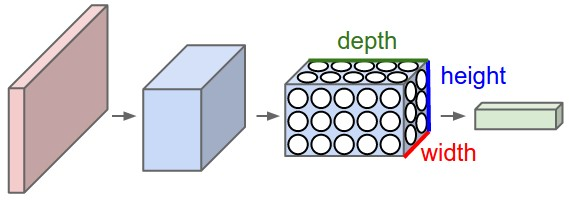
\includegraphics[scale=.5]{images/cnn.jpeg}
	\caption{Neuroni di una CNN}
	\label{fig:cnn}
\end{figure*}

\begin{figure*}[h]
	\centering
	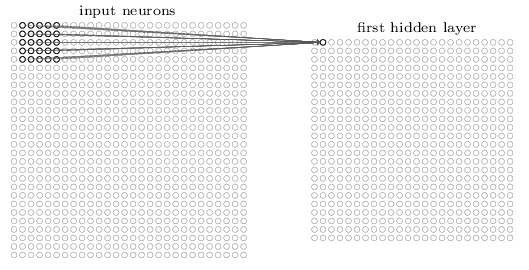
\includegraphics[scale=.5]{images/hlayer.jpeg}
	\caption{}
	\label{fig:hlayer}
\end{figure*}

\section{Perchè non funziona}\label{}
	\subsection{Il sospetto}
		A livello intuitivo
		\begin{table*}[h]
			\centering
			\caption{asd}
			
			\label{tab:gerarchia}
		\end{table*}
		\begin{table*}[h]
			\centering
			\caption{asd}
			\label{tab:pgm}
			
		\end{table*}
	
	
	\subsection{Perchè}
		La "dimostrazione".
		
\section{Prove}
	\subsection{Gioco successo}
	
	\subsection{Gioco fallimento}
		
\section{Agenti Alternativi}\label{}
	Spiegare l'evoluzione dell'argomento.

	\begin{figure*}[h]
		\centering
		%\includegraphics[scale=.4]{img/rnn.png}
		\caption{asd}
		\label{fig:unroll}
	\end{figure*}

	\begin{figure*}[h]
		\centering
		%\includegraphics[scale=.5]{img/lstm.png}
		\caption{asd}
		\label{fig:lstm}
	\end{figure*}

	\begin{figure*}[h]
		\centering
		\begin{subfigure}[b]{.496\textwidth}
			%\includegraphics[width=\textwidth]{img/inside-lstm.png}
			\caption{asd}
		\end{subfigure}
		\begin{subfigure}[b]{.496\textwidth}
			%\includegraphics[width=\textwidth]{img/inside-lstm2.png}
			\caption{Parametri calcolati nelle ultime fasi}
		\end{subfigure}
		\caption{asd}
		\label{fig:parmap}
	\end{figure*}
	
	\begin{equation}\label{eq:ft}
		f_t = \sigma(W_f \cdot [h_{t - 1}, x_t] + b_f)
	\end{equation}
	
	\begin{figure*}[h]
		\centering
		%\includegraphics[scale=.3]{img/seqs.jpeg}
		\caption{Problemi \textit{sequence-to-sequence} trattabili con le \texttt{RNN}}
		\label{fig:seqs}
	\end{figure*}
	\begin{figure}
		\centering
		%\includegraphics[scale=.26]{img/blstm.png}
		\caption{Architettura astratta di una rete \texttt{BLSTM}}
		\label{fig:blstm}
	\end{figure}
	\begin{figure*}[ht!]
		\centering
		\caption{Costruzione del modello con \texttt{Keras}}
		%\lstinputlisting[language=Python]{code/seq.py}
		\label{fig:modelcode}
	\end{figure*}
	\begin{table*}[]
		\centering
		\caption{Risultati ottenuti in seguito al lavoro di progetto, confrontati con il modello \texttt{LDCNF}.}
		\label{tab:results}
		
	\end{table*}
	
	\section{Conclusioni}	
	
\begin{thebibliography}{99}	
	\bibitem{bib:dqn}
		Volodymyr Mnih, Koray Kavukcuoglu and David Silver,
		\newblock \emph{Human-level control through deep reinforcement learning},
		2015.
		
	\bibitem{bib:chollet2015keras}
		Chollet, Fran\c{c}ois,
		\newblock \emph{Keras},
		\url{https://github.com/fchollet/keras},
		2015

\end{thebibliography}

\end{document}
